\chapter{IMPROVED DUAL-SIM APPROACH TO GATESIM}
\label{chap:dualsim.tex}
After analyzing limitations associated with \emph{early dual-sim approach} it could be inferred that the main cause of inefficiency was the method used to capture, store, and apply test-vectors onto the netlist. Analyzing limitations associated with \emph{co-sim approach}, it could be inferred that the cause was bulky test-bench components associated with RTL simulations. Hence an improved solution would contain minimal testbench components retained and have an efficient method to capture, store, and apply test-vectors. 

Test-vectors are nothing but signal values at specific point in time. There are already different formats to store this information efficiently. FSDB \nomenclature{FSDB}{Fast Signal Database} is one such format. Hence it was suggested to improve gatesim methodology using FSDB itself as the format to store test-vectors. The proposed solution should also improve on

\begin{description}
	\item[Storage requirements]: Ensuring that storage resources are effectively used
	\item[Turn-around times]: Should avoid re-build for different test-vectors
\end{description}

FSDB\cite{SS:Verdi} or Fast Signal Database is a signal data file, similar to VCD\cite{ieee:v:2005} \nomenclature{VCD}{Value Change Dump} but much more compact. This format is in wide use across industry. Quick analysis revealed that FSDB as input test-vectors could be accomplished. Existing API's \nomenclature{API}{Application Programming Interface} provided by Verdi\cite{SS:Verdi} tool set for FSDB format could be used to retrieve values from FSDB. PLI$/$VPI\cite{ieee:v:2005} could be used to drive stimulus onto netlist.


The improved methodology becomes a dual-simulation methodology with two separate simulations.
\begin{enumerate}
	\item First simulation with non-gatesim components to generate the test-vectors in FSDB format.
	\item Second simulation with only gatesim components with capability to apply test-vectors from FSDB directly.
\end{enumerate}



\section {IMPROVED METHODOLOGY}
\label{sec:dualsim:im}
In dual simulation methodology the idea is to have two seperate simulations unlike co-sim. Both these simulations are completely independet except for the stimulus vector file. In the first unmodified RTL simulation (together with test bench components) dump is enabled in FSDB format. This FSDB dump is used as test-vectors for the following netlist simulation. In co-simulation methodology the same test bench will provide stimulus to RTL and netlist. ~\figurename{~\ref{fig:gatesim_flow.ps}} shows a flow diagram of proposed dual-sim methodology.  
\begin{figure}[h]
\centering
\includegraphics[scale=0.55]{./figures/gatesim_flow.ps}
\caption{Dual Sim}
\label{fig:gatesim_flow.ps}
\end{figure}

Stages associated with this methodology are
\begin{description}
	\item[RTL simulation] RTL simulation along with test bench components is already being done as part of functional verification. For gatesims, no changes are required except that the simulation signals needs to be dumped into FSDB, through runtime switches. Such FSDB stimulus vectors have to be generated for every stimulus envisioned to be applied onto the netlist. Note that once generated, the stimulus could be reused for repetitive netlist simulations.
	\item[Gatesim infrastructure] As in the case of co-simulation, gatesim files need to be generated from files obtained from LEC flow. Same infrastructure used in co-sim is used for this and hence no additional effort is required when the methodology is modified. Note that this step needed to be done only once.
	\item[Gatesim Build] Gatesim build could be obtained after compiling and elaborating the design netlist and infrastructure files with a simulator. The build would be devoid of RTL design and non-gatesim verification infrastructure. Note that this step needed to be done only once.
	\item[Gatesim simulation] Run all envisioned stimulus vectors onto the netlist.
\end{description}


{\bf VCS}: VCS is a high-performance Verilog simulator that  incorporates advanced, high-level abstraction verification  technologies into a single open native platform. VCS provides a fully featured implementation of Verilog language as defined in the {\it IEEE Standard Hardware Description Language} based on {\it Verilog Hardware Description Language (IEEE Std 1364-1995)} and {\it Standard Verilog Hardware Description Language (IEEE Std 1364-2001)}. It supports almost all verification, design and assertion constructs of {\it System Verilog}. It also provides native interfaces like DKI\nomenclature{DKI}{Direct C Kernel Interface} etc. VCS is a compiled code simulator and is widely considered as one of the advanced simulators avialable in the industry.

For this project we had used {\it VCS Verilog simulator} developed by {\it Synopsys Inc.} for RTL as well as netlist simulations. \figurename{\ref{fig:RTL_sim.eps}} is a self explainatory depction of RTL simulation. The implementation details of this methodology is detailed in following sections. 

\begin{figure}[h]
\centering
\includegraphics[scale=0.5]{./figures/RTL_sim.ps}
\caption{RTL Simulation}
\label{fig:RTL_sim.eps}
\end{figure}


\subsection{NETLIST SIMULATION FLOW}
\figurename{\ref{fig:netlist_sim.ps}} shows netlist simulation flow. Process~\textcircled{a} is generation of FSDB stimulus, which is already explained in Section~\ref{sec:dualsim:im}. Process~\textcircled{b} is intricated and is detailed in Section~\ref{sec:dualsim:sa}. Remaining process stages are explained here.

\begin{figure}[h]
\centering
\includegraphics[scale=0.65]{./figures/netlist_sim.ps}
\caption{Netlist Simulation}
\label{fig:netlist_sim.ps}
\end{figure}

Process stages of netlist simulation flow are:
\begin{enumerate}
	\item Obtain test-vectors in FSDB format
	\item Drive stimulus onto a dummy-RTL
	\item Dummy-RTL drives stimulus onto netlist
	\item Apply appropriate force signals from FSDB on to the dummy-RTL, which then forces it onto appropriate netlist nodes.
	\item Accomplish verification goals by clock-cycle-based-comparators connected between golden RTL reference and corresponding netlist nodes.
\end{enumerate}

\subsection{DUMMY-RTL}
When test-vectors were applied from FSDB to {\it Verilog} design, it was found that VPI/DKI method of stimulus application is not suitable when driving {\it Verilog} nets. Nets have special behaviour that they needs to be continuously dirven, which in the case of VPI/DKI is through forcing the net. But it was found to have flaky behaviour. Hence it was decided to create a ``dummy-RTL'' module that would contain all the signals those need to be export out of FSDB. These signals would have same size as their actual counterparts but be of type {\it Verilog} ``reg''. Test-vectors from FSDB would be applied to these signals inside dummy-RTL. Listing~\ref{nl:dualsim:dummy} shows a code snippet of dummy-RTL module (Process~\textcircled{c} in \figurename{\ref{fig:netlist_sim.ps}}). All wires, IO signals are of type ``reg'' in dummy-RTL module.

\lstset{language=Verilog,
basicstyle=\footnotesize,
frame=shadowbox,
breaklines=true}          
\begin{lstlisting}[frame=single, caption=Dummy RTL Module, label=nl:dualsim:dummy]  
module dummy_RTL();
	reg input_signal_1;
	reg input_signal_2;
	 -
	 -
	reg input_signal_n;
					
	reg output_signal_1;
	reg output_signal_2;
	 -
	 -
	reg output_signal_m;
endmodule
\end{lstlisting}



\subsection{SIMULUS APPLICATOR}
Stimulus from dummy-RTL module is applied onto netlist by {\it Verilog} by connecting ports of netlist while instantiation at gatesim test-bench.  Listing~\ref{nl:dualsim:inst} gives a snippet of this Verilog instantiation of netlist module. There could be certain forces required in certain logic inside netlist, which is accomplished through {\it Verilog}'s ``force'' statement. These forces could be for initialisation, fuses or for hastening reset release.

\lstset{language=Verilog,
basicstyle=\footnotesize,
frame=shadowbox,
breaklines=true}          
\begin{lstlisting}[frame=single, caption=Verilog Instantiation, label=nl:dualsim:inst]  
netlist GATE (
	.input_signal_1 (dummy_RTL.input_signal_1);
	.input_signal_2 (dummy_RTL.input_signal_2);
	.input_signal_3 (dummy_RTL.input_signal_3);
	.input_signal_4 (dummy_RTL.input_signal_4);
			-
			-
	.input_signal_n (dummy_RTL.input_signal_n);

	.output_signal_1();
	.output_signal_2();
			-
			-
	.output_signal_m();
	);

\end{lstlisting}



\subsection{NETLIST SIMULATION}
Process~\textcircled{e} is simulation with netlist testbench components. These components are reused form of co-simulation methodology's netlist components (Section~\ref{sec:method:csgs}), with references of actual RTL paths changed to {\it Dummy-RTL}'s paths. Waveform dump needs to be enabled during simulation to enable debug in case of failure. Reference RTL waveform dump file is already available for the user.


\subsection{FUNCTION COMPARATORS}
Process~\textcircled{f} are a set of comparators those keep checking the behaviour of netlist with respect to RTL on every clock-cycle. Generally the comparision is made on respective active clocks, well after all signal changes have died down. The reference RTL signal is available in the dummy-RTL. Comparators may also consider certain important internal nodes, hence those have to be available in dummy-RTL as well. Listing~\ref{nl:dualsim:comp} is a code snippet representing a single comparator. Whenever compare fails, a ``miscompare'' information is written on to simulation transcript, that would aid debug. When test completes without any ``miscompare'' report, then test is said to have completed without failures.

\lstset{language=Verilog,
basicstyle=\footnotesize,
frame=shadowbox,
breaklines=true}          
\begin{lstlisting}[frame=single, caption=Cycle Based Comparison, label=nl:dualsim:comp ] 
//comparator for output signal 1 
always @(negedge CLK) begin
#1
 if (GATE.output_signal_1 != dummy_RTL.output_signal_1)
    $display(``Mismatch for signal 1'')`;
 end
end

\end{lstlisting}


\section{STIMULUS APPLICATOR}
\label{sec:dualsim:sa}
Process~\textcircled{b} is a layered software infrastructure for the purpose of stimulus application onto the dummy-RTL. ~\figurename{~\ref{fig:fsdb.ps}} shows four different layers of the applicator. Together they accomplish transporting vector stimulus from FSDB file and finally delivering it to the netlist simulation. The first layer used to access FSDB file is provided by {\it Verdi} tool itself. It is available as a pre-built object\cite{Verdi:FsdbReader}, which could be linked with. The remaining three-layers of the infrastructure has been developed as part of this project and implemented as {\it C} and {\it C++} code.

\begin{figure}[h]
\centering
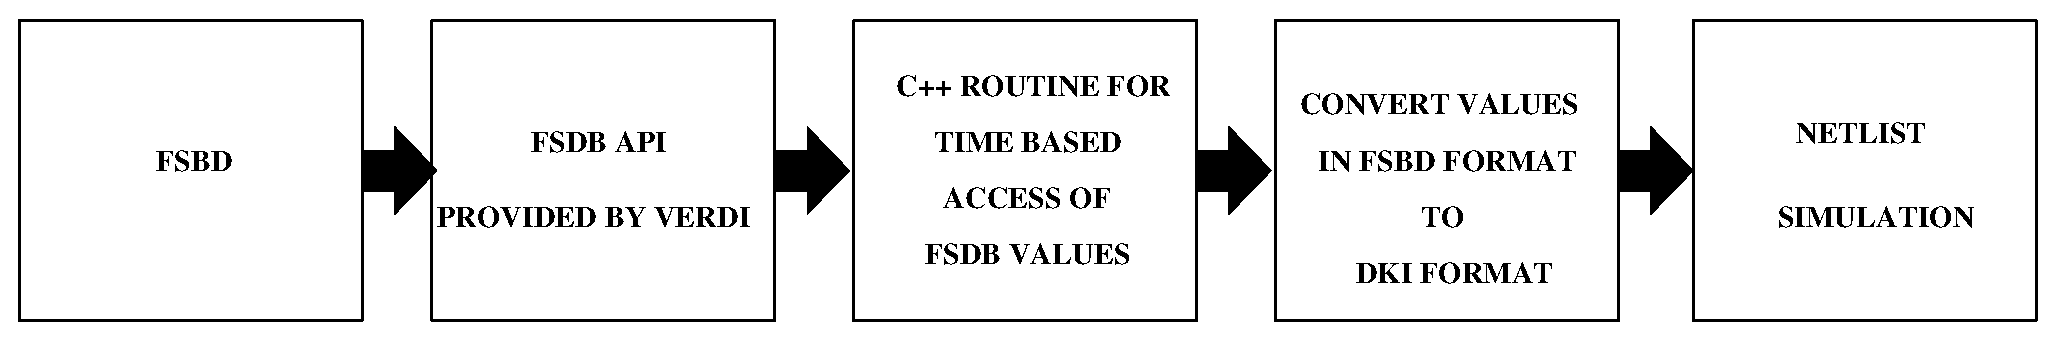
\includegraphics[scale=0.65]{./figures/fsdb.ps}
\caption{Accessing FSDB Signals}
\label{fig:fsdb.ps}
\end{figure}

\subsection{EXTRACTING STIMULUS}
FSDB is a binary file format for storing signal value change information. This format commonly used across the {\it Verdi} toolset and no other program has enough information to decode data from those files. But {\it Verdi} toolset, provides APIs\cite{Verdi:FsdbReader} \nomenclature{API}{Application Programmer's Interface} to be interfaced with. This project make use of those APIs, to accomplish desired task of accessing design signals at any point in time.

\begin{figure}[h]
\centering
\includegraphics[scale=0.65]{./figures/verdi.ps}
\caption{API For Accessing FSDB Signals}
\label{fig:verdi.eps}
\end{figure}

In order to successfully extract signal values from stored FSDB file the following needs to be done
\begin{enumerate}
\item[Handle FSDB file] In this process approprite FSDB file needs to be ``opened'' and be ``closed'' after all operations are completed. {\it Verdi} provides routines \texttt{ffrOpen()/ ffrOpen2()} and \texttt{ffrClose()} for these purposes respectively.
\item[Obtain signal handle] In this process handle to signals of interest needs to be obtained through APIs. Sample routine \texttt{MyTreeCBFunc}\cite[p.~3]{Verdi:FsdbReader} is already provided by {\it Verdi}.
\item[Access signal values] Once signal handle is obtained, the signal's value at this point in time could be obtained by routine \texttt{ffrGetVC()}.
\end{enumerate}

\subsection{TIME BASED TRAVERSAL}
\begin{figure}[h]
\centering
\includegraphics[scale=0.61]{./figures/time_access.ps}
\caption{Time Based Application of Stimulus}
\label{fig:dualsim:tbas}
\end{figure}

\figurename{\ref{fig:dualsim:tbas}} shows sequences of actions that would occur during simulation. At any simulation time `M', it would be required to apply the stimulus to all signals of interest. After  this, control is transferred to simulator which computes  the states values at time `M'. The event driven simulation  would proceed in this fashion for all subsequent event times until it reaches the next stimulus point `N'. Series of actions that took place for time `M' would be repeated for time `N'  and so forth.

List of RTL signals those need to be extracted would be refined over time, as netlist becomes stable. In this particular application, it would  be required  to obtain values of all signals of interest at the desired  instant. This type of traversal is called as time-based-traversal. Sample routine \texttt{tb.cpp}\cite[p.~28]{Verdi:FsdbReader} is already provided by {\it Verdi}. In this application, a larger C++ infrastructure is required to be built since
\begin{enumerate}
\item Number of RTL signals those needs to be extracted is huge. Hence a seperate data structure is required.
\item Accessing of signal values in time-based fashion could be abstracted out.
\item Signal sizes vary from 1 to hundredes, so handling of different sized signals could be made uniform by {\t C++} routine abstraction.
\end{enumerate}


\subsection{VALUE CONVERSION TO DKI}
FSDB exports signals values in its custom 8-bit format, but that can't be used directly by any simulator. These values needs to get converted to a format that could be understood by the simulator. {\it Verilog} language\cite{ieee:v:2005} provides many standard interfaces such as PLI, VPI (or PLI 2.0) for this purpose. The drawback with these standard interfaces are that they are too slow when huge vectors are in consideration (like gatesims). Conversions to and from string based format is very timeconsuming as it was observed.

In order to overcome these limitations, VCS provides a non-standard interface called as DKI \nomenclature{DKI}{Direct-C Kernel Interface}. This interface has the advantage of less simulation overhead and smaller memory footprint compared to VPI interface. Hence DKI was choosen for this project.

%\begin{figure}[h]
%\centering
%\includegraphics[scale=1]{./figures/dki.ps}
%\caption{FSDB Format to DKI format}
%\label{fig:dki.eps}
%\end{figure}

Signal values could be retrived through {\it Verdi} APIs, as listed in speudo-code in Listing~\ref{nl:dualsim:rvf}.

\lstset{language=C++,
basicstyle=\footnotesize,
frame=shadowbox,
breaklines=true}          
\begin{lstlisting}[frame=single, caption=Retrieving Values from FSDB,label=nl:dualsim:rvf] 
  byte_T *vc_ptr;
  /* vc_ptr should be assigned to particular signals value change */

  // convert verilog bits to unsigned int
  uint retVal=0;
  uint8 bit;
  for (int i=0; i<=(msb-lsb); i++) {
    bit = vc_ptr[i+LBit-msb];
    retVal = (retVal<<1)
           | (bit==FSDB_BT_VCD_1 || (bit==FSDB_BT_VCD_X));
  }
\end{lstlisting}
\renewcommand{\lstlistingname}{Code}

DKI provides direct interface to internal representation of simulator object. Signal values retrieved from FSDB could be assigned to VCS's object as per instructions in {\it VCS User Guide}\cite[Section~C~Language~Interface>~Direct~C]{VCS:vcs.pdf}.

\subsection{INTERACTION WITH SIMULATOR}
Having obtained vector values and having the capability to apply it to the simulator, the final part of stimulus application is to have the ability to stop simulator at will and trigger new vector application. Since advanced simulators like VCS are event based, the interruption on simulation  has to be done on need basis rather than on every unit dealy. This could be accomplished with the use of standard simulator interfaces such as VPI callbacks. Enough documentation on this subject could be found in standard texts\cite{ss:pli:1999}~\cite{sm:pli:1999} and online\cite{wiki:2013:VPI}~\cite{aw:2013:VPI}. Listing~\ref{nl:dualsim:svc} shows a snippet of code that could be used to schedule a callback from simulator by specifying the delta-delay.

%\begin{newlisting}[caption=Scheduling a VPI callback,label=nl:dualsim:svc]
\lstset{language=C++,
basicstyle=\footnotesize,
frame=shadowbox,
breaklines=true}          
\begin{lstlisting}[frame=single, caption=Scheduling a VPI callback,label=nl:dualsim:svc] 
  vpiHandle  cbHandle;
  s_vpi_time vpiTimeObj;
  s_cb_data  cbData;

  vpiTimeObj.type = vpiSimTime;
  vpiTimeObj.low  = delay & 0xffffffff;
  vpiTimeObj.high = delay >> 32;

  cbData.reason    = cbAfterDelay;
  cbData.cb_rtn    = GlobalCallbackSyncFunc;
  cbData.time      = &vpiTimeObj;
  cbData.value     = NULL;
  cbData.obj       = NULL;
  cbData.user_data = (PLI_BYTE8*) vpiCallbackPtr;

  cbHandle = vpi_register_cb(&cbData);
  vpi_free_object(cbHandle);
\end{lstlisting}

Delta-delay is the simulation time difference between next stimulus point with respect to the current simulation time. Current simulation time could be obtained through VPI \verb|vpi_get_time()| routine. The next stimulus point could be obtained through fsdb routines. Stimulus application is acheived by continously progressing to next stimulus point followed by application of stimulus, as shown in snippet Listing~\ref{nl:dualsim:sar}.

%\begin{newlisting}[caption=Stimulus Applicator Routine,label=nl:dualsim:sar]
\lstset{language=C++,
basicstyle=\footnotesize,
frame=shadowbox,
breaklines=true}          
\begin{lstlisting}[frame=single, caption=Stimulus Applicator Routine,label=nl:dualsim:sar] 
  static fsdbXTag cur_time, nxt_time;

  /* Find the next time instant in FSDB and cause a callback at that time */
  while (FSDB_RC_SUCCESS == tb_trvs_hdl->ffrGotoNextVC()) {
    tb_trvs_hdl->ffrGetXTag(&nxt_time);
    if ((cur_time.hltag.L != nxt_time.hltag.L) || (cur_time.hltag.H != nxt_time.hltag.H)) break;
  }
  if ((cur_time.hltag.L != nxt_time.hltag.L) || (cur_time.hltag.H != nxt_time.hltag.H)) {
    uint64 delta = (((uint64)(nxt_time.hltag.H - cur_time.hltag.H))<<32) | (nxt_time.hltag.L - cur_time.hltag.L);
    ScheduleAfterDelayCallback(delta, this); /* This routine would be called back again after the delta */
  }

  /* Do assignments */
  for (uint32 ui=0; ui<num_sigs; ui++) {
    /* Assign FSDB value of signal to DKI object */
  }

  /* Finish if no more stimulus */
  if ((cur_time.hltag.L == nxt_time.hltag.L) && (cur_time.hltag.H == nxt_time.hltag.H)) {
    /* Finish simulation */
  }

  /* Will be used during recursive call */
  cur_time = nxt_time;
\end{lstlisting}

%\begin{figure}[h]
%\centering
%\includegraphics[scale=1]{./figures/cpp.ps}
%\caption{C++ Routine for FSDB Signal Extraction}
%\label{fig:cpp.eps}
%\end{figure}
%
%The C++ infrastructure will open the FSDB file and initiate a playback through the file. Whenever a signal that is attached using APIs changes, the C++ will identify this and will ensure the changed value is made available to the netlist simulation.  Figure x shows the complete flow of the C++ routine developed for FSDB signal access, conversion and application onto Verilog component.
%A set of RTL signal accessed at time based manner and applied onto netlist is effectively doing the job of test-vectors as vectors are nothing but signal values at different instants of time.
%Once signals are accessed from FSDB file by API's and C++ routine developed next step is applying it onto netlist. However Verilog based netlist cannot directly interact with extracted FSDB format objects. For this a conversion stage is required.  
%
%Whenever the C++ moves in time and identify a change in signal value in FSDB signal, an assign statement will assign the new FSDB signal value to DKI signal object.  These DKI signals can drive Verilog signals by using "{\emph Attach}" routine provided by API, that ties together DKI object with RTL signal. 
%
%In the previous section we have discussed extracting FSDB, accessing it in a time based manner and converting it to a format that can interact with Verilog. Next step is using these signals for netlist simulation.

